\chapter{Implementation}\label{ch:Implementation} 
In this chapter, I will present my contributions to this work and go over the technical side of
things. First off, we need to discretise the theory introduced in chapter \ref{ch:Theory} in order
to implement the corner detection and inpainting algorithms. To do that, we need to talk about
discrete images and the method of finite differences to approximate image derivatives.
After that we shortly talk about discretisation of diffusion processes which we need to implement
the inpainting/restoration part to test the mask we chose.\\  
In the second chapter I will introduce corner regions as an essential concept to this work and talk
about the additions we made to the corner detection algorithm in order to select the most valuable
corners for our inpainting mask.\\
All the source code is written in pure C and can be found in the appendix.
The initial corner detection algorithm as well as the code for the inpainting alogorithm was given
to me courtesy of Joachim Weickert.

\section{Discretisation}\label{sec:Discretisation}

Since reality is not infinitely fine, things such as infinitesimal calculations as seen in 
calculus, e.g. differentation of functions, can not be applied to the real world directly.
This is a problem, because digital images are inherently not continuous as they contain only a
finite number of pixels. 
We could have also solved the theoretical problem in a discrete domain but that would have 
been much more troublesome.
That is why we rather develop a continuous theory and then discretise it later to actually
implement the ideas as algorithms.

\subsection{Discrete images}
Let $f:\Omega \rightarrow \mathbb{R}$ be an image where $\Omega
:= (0, n_x)\times(0, n_y) \subset \mathbb{R}^2$ as defined in section \ref{sec:Basics}. To
\textit{sample} the image, i.e. to discretise the image domain, we assume that all pixels lie on a
rectangular equidistant grid inside $\Omega$, where each cell in the grid has a size of $h_x
\times h_y$.
That yields $N_x := n_x/h_x$ pixels in x- and $N_y := n_y/h_y$ pixels in
y-direction.
That being said, we define the pixel $u_{i,j}$ at grid location $(i, j)^\top$ as
\begin{equation}
    u_{i, j} := u(ih_x, jh_y)\qquad \forall(i ,j) \in \{1,\dots,N_x\}\times\{1,\dots,N_y\}
\end{equation}
With that approach, the pixels are defined to lie on the crossing of the grid lines.
An alternative idea defines the pixels to lie in the centre of each cell, i.e. at location 
$((i-\frac{1}{2})h_x,\ (j- \frac{1}{2})h_y)^\top$.
As a sidenote, the cell sizes in either direction are pretty much always assumed to be 1 in 
practice. 
But to keep the theory as universal as possible, we will use $h_x$ and $h_y$ instead.\\
Sampling of the spatial domain is not the only step necessary to fully discretise an image. We also have
to discretise the \textit{co-domain} or \textit{grey-value-domain}. In theory our grey value domain
is just $\mathbb{R}$, but since this is rather unpractical, we limit it to $[0, 255]$. This step of
the discretisation process is also called \textit{quantisation}.

\subsection{Numerical differentiation}

Image derivatives are essential to image processing as seen in the previous chapter. Therefore we
need a way to compute them even on discrete images. To compute the gradient or in the simpler case
just the derivative of a discrete function, one generally uses so called \textit{finite difference
schemes}. Such a scheme is normally derived from the \textit{Taylor expansion} of the continuous
function. For example, we want to compute the first derivative of a 1D function $f:\mathbb{R}
\rightarrow \mathbb{R}$.
The Taylor expansion of \textit{degree $n$} of this function around the point $x_0\in\mathbb{R}$ is given by 
\begin{equation}
    f(x) = T_n(x, x_0) + \mathcal{O}(h^{n+1})
\end{equation}
where $\mathcal{O}(h^{n+1})$ describes the magnitude of the leading error term and as such the
\textit{approximation quality} of the Taylor series.
The actual Taylor series is defined as
\begin{equation}
    T_n(x, x_0) = \sum\limits_{k=0}^{n} \frac{(x-x_0)^k}{k!}f^{(k)}(x_0)
    \footnote{$f^{(k)}$ denotes the $k$-th derivative of the function $f$}
\end{equation}
A finite difference scheme generally uses a weighted sum of neighbouring values to compute the
desired derivative expression. In our example, we want to derive a scheme to compute the first
derivative of $f_i$ using its neighbours $f_{i-1}$ and $f_{i+1}$, i.e.
\begin{equation}
    f_i' \approx \alpha f_{i-1} + \beta f_i + \gamma f_{i+1}
\end{equation}
We can now describe $f_{i-1}$ and $f_{i+1}$ in terms of their Taylor expansion around $f_i$: 
\begin{align}
    f_{i-1} &= f((i-1)h) \notag\\
            &= T_n((i-1)h, ih) + \mathcal{O}(h^{n+1})\notag\\
            &= \sum\limits_{k=0}^{n}\frac{(-h)^k}{k!}f_i^{(k)}+ \mathcal{O}(h^{n+1})\\
    f_{i+1} &= \dots = \sum\limits_{k=0}^{n}\frac{h^k}{k!}f_i^{(k)}+ \mathcal{O}(h^{n+1})
\end{align}
If we now choose a concrete value for $n$ (here $n=5$) we can actually compute the approximation:
\begin{align}
    f_{i-1} &= f_i - hf_i' + \frac{h^2}{2}f_i'' - \frac{h^3}{6}f_i''' + \frac{h^4}{24}f_i'''' -
    \frac{h^5}{120}f_i''''' + \mathcal{O}(h^6)\label{eq:fi-1}\\
    f_{i+1} &= f_i + hf_i' + \frac{h^2}{2}f_i'' + \frac{h^3}{6}f_i''' + \frac{h^4}{24}f_i'''' +
    \frac{h^5}{120}f_i''''' + \mathcal{O}(h^6)\label{eq:fi+1}
\end{align}
The next step is the \textit{comparison of coefficients}, we insert
\eqref{eq:fi-1} and \eqref{eq:fi+1} into the equation 
and solve the arising linear system of equations for $\alpha,\beta,\gamma$.
\begin{align}
    0\cdot f_i + 1\cdot f_i' + 0\cdot f_i'' \overset{!}{=} \alpha f_{i-1} + \beta f_i + \gamma
    f_{i+1}
\end{align}
After the substitution, the right hand side becomes
\begin{align}
    &\alpha \left(f_i - hf_i' + \frac{h^2}{2}f_i''\right) + \beta f_i + \gamma\left(f_i + hf_i' + \frac{h^2}{2}f_i''\right)\notag\\
    = &\left(\alpha+\beta+\gamma\right)f_i + h\left(-\alpha+\gamma\right)f_i' + \frac{h^2}{2}\left(\alpha+\gamma\right)f_i''
\end{align} 
Note that for the comparison of coefficients it suffices to use the first 3 summands of the
approximation.
The linear system defined by the above equation
\begin{equation}
    \begin{pmatrix}
        1&1&1\\
        -1&0&1\\
        1&0&1
    \end{pmatrix}
    \begin{pmatrix}
        \alpha\\
        \beta\\
        \gamma
    \end{pmatrix}
    =
    \begin{pmatrix}
        0\\
        \frac{1}{h}\\
        0
    \end{pmatrix}
\end{equation}
has the solutions $\alpha = -\frac{1}{2h}, \beta = 0, \gamma = \frac{1}{2h}$.
This yields the approximation 
\begin{equation}
    f_i'\approx\frac{f_{i+1} - f_{i-1}}{2h}
\end{equation}
To find out how good this scheme is, we re-insert \eqref{eq:fi-1} and \eqref{eq:fi+1} to get
\begin{align}
    \frac{f_{i+1} - f_{i-1}}{2h}= -&\frac{1}{2h}\left(f_i - hf_i' + \frac{h^2}{2}f_i'' - \frac{h^3}{6}f_i''' + \frac{h^4}{24}f_i'''' -
    \frac{h^5}{120}f_i''''' + \mathcal{O}(h^6)\right) + \notag\\
     &\frac{1}{2h}\left(f_i - hf_i' + \frac{h^2}{2}f_i'' - \frac{h^3}{6}f_i''' + \frac{h^4}{24}f_i'''' -
    \frac{h^5}{120}f_i''''' + \mathcal{O}(h^6)\right)\notag
\end{align}
Expanding and simplifying yields
\begin{align}
        \frac{f_{i+1} - f_{i-1}}{2h} &= f_i' + \underbrace{\frac{h^2}{6}f_i'' + \frac{h^4}{30}f_i'''' +
        \mathcal{O}(h^5)}_\text{quadratic leading error term}\notag\\
            \Rightarrow \frac{f_{i+1} - f_{i-1}}{2h} &= f_i' + \mathcal{O}(h^2)
\end{align}
This means that the error of our approximation is quadratic in the grid size. 
We also say that this approximation has a \textit{consistency order} of 2. Note that for such an
approximation to be reasonable, it has to have at least consistency order 1. Otherwise, it is
not guaranteed that the error term diminishes if we send the grid size $h$ to 0.\\
The scheme derived above is also called \textit{central difference scheme}. Not that there are
other schemes such as \textit{forward} and \textit{backward} differences, but for the most part, we
will only use central differences since it provides us with the highest consistency
order out of all three. 
\begin{align}
    f_i' &= \frac{f_i - f_{i-1}}{h} + \mathcal{O}(h)&\textnormal{(backward differences)}\notag\\
    f_i' &= \frac{f_{i+1} - f_i}{h} + \mathcal{O}(h)&\textnormal{(forward differences)}\notag
\end{align}
\subsection{Numerical schemes for diffusion}
\section{Corner regions}\label{sec:Contribution}
Our starting point for the detection of the most relevant corners was the classic Foerstner-Harris
corner detector based on the structure tensor (cf. section \ref{sub:Corner}). 
\begin{equation}
    \frac{\textnormal{det}(\boldsymbol J_\rho)}{\textnormal{tr}(\boldsymbol J_\rho)} =
    \frac{\lambda_1\lambda_2}{\lambda_1 + \lambda_2}\label{def:Harris}
\end{equation}
With that we build on the method that Zimmer \cite{zimmer07} examined in 2007. They chose the
Foerstner-Harris detector because it is very accurate and simulatneously not as computationally
invested as the Tomasi-Kanade detector that requires to compute both eigenvalues of the structure
tensor using a principal axis transformation.\\
But unlike in \cite{zimmer07}, we aim to to not just keep a small outline around the most important
corners but increase the radius and keep a disc of pixels around each of them. 
\begin{equation}
    \texttt{corner\_region}_R(\boldsymbol x) := \lbrace \boldsymbol y \in \Omega\ : \ \lVert \boldsymbol
    x - \boldsymbol y\rVert_2^2 \leq R^2 \rbrace
\end{equation}
One problem of this approach that was already apparent in \cite{zimmer07} is the sparsity of
corners or similar features in images. Therefore, we had to come up with a solution to somehow
solve this issue in order to create masks with which we can reconstruct the image reasonably 
well.
Another issue is that we have to limit the number of corners depending on the size of the corner
regions since too many corners would result in a very dense mask not very suitable and/or
useful for image compression. 
To solve these issues reasonably well, we introduced two additional steps to the corner detection
process.
\subsection{Circular non-maximum suppression}\label{sub:Suppression}
In the original version of the Foerstner-Harris corner detector, corners are detected as the local
maxima of the cornerness measure \eqref{def:Harris}. However, in this method, the local maxima were
only determined in a 4- or 8-neigbourhood. This works fine in a setting where corner regions are
very small as they were in \cite{zimmer07}. When using larger regions however, this might create a
very unique problem.\\
What we noticed when using the usual 8-neighbourhood non-maximum suppression together with larger
circular corner regions is that in some
images where multiple corners were located right next to each other this approach would create
masks with many overlapping corner regions in a single spot and no regions in other places. To
counteract this, we introduced \textit{circular non-maximum suppression} (\textbf{CNMS}).\\
\begin{figure}
    \begin{lstlisting}[language=Python]
def circular_suppression(harris, (x, y), r, out):
    ''' Circular non-maximum suppression at location (x,y) with radius r.
    Parameters:
        -harris: Harris measure map
        -(x, y): current location
        -r: radius of corner regions
        -out: map of accepted corners after suppression
    '''
    for x', y' in circle(x, y, r):
        if harris[x',y'] > harris[x,y]:
            # The current location is not a maximum
            out[x, y] = 0
            return
    # Current location is a maximum, keep the region around it
    out[x, y] = harris[x, y]
    return 
    \end{lstlisting}
    \caption{Pseudo-Code for circular non-maximum suppression}
\end{figure}
The idea behind this addition is that in larger corner regions, one might have multiple 
important corners in a single corner region.
Now, instead of creating a disc around every single one of these corners, we checked if there 
would be another maximum in an imaginative circle around this corner. 
If this is the case, we disregard this corner region since the current corner is already 
contained in another region.
Using this approach, we were able to create masks with little to no overlap between the
corner regions. However, this introduced one problem that we were not able to fix properly as
discussed in section \ref{sec:Discussion}.
% Examples for circular non-maximum suppression (CNMS) against normal non-maximum suppression
After circular non-maximum suppression, we applied \textit{percentile thresholding} to make sure,
that, out of the set of corners we just detected, we only keep the most important corner regions. 

\begin{figure}
    \centering
    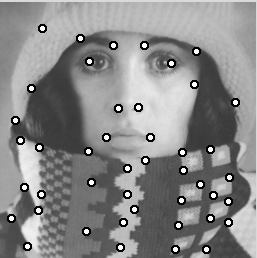
\includegraphics[width=0.31\linewidth]{../Images/trui_corners_cnms.png}
    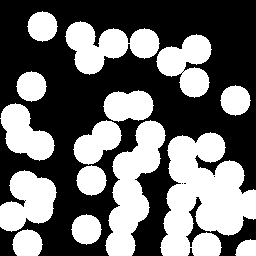
\includegraphics[width=0.31\linewidth]{../Images/trui-mask_cnms.png}
    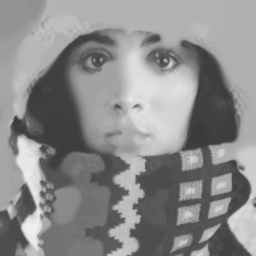
\includegraphics[width=0.31\linewidth]{../Images/trui-inpaint_cnms.png}\\
    \vspace{0.2cm}
    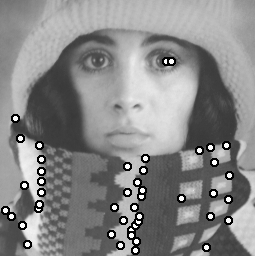
\includegraphics[width=0.31\linewidth]{../Images/trui_corners_non_cnms.png}
    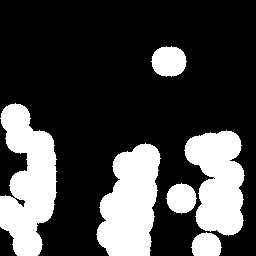
\includegraphics[width=0.31\linewidth]{../Images/trui-mask_non_cnms.png}
    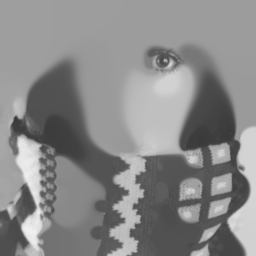
\includegraphics[width=0.31\linewidth]{../Images/trui-inpaint_non_cnms.png}
    \caption{Effect of circular non maximum suppression on spread of corners across the image.
        \textbf{Top row:} Position of corners, inpainting mask and inpainting results
        \textbf{with} CNMS.
\textbf{Bottom row:} Position of corners, inpainting mask and inpainting results \textbf{without} CNMS.
    Corner detection with Foerstner-Harris corner detector, $\sigma=1,\rho=2.5,R=15$ and a
percentile of 0.5}
\end{figure}

\TODO{Redo this section for the new thresholding}
\subsection{Percentile thresholding}\label{sub:Percentile}
In the classic version of Harris corner detection, an artificial threshold parameter $T$ is
introduced to weed out `bad' corners. This parameter however is fairly sensible to the input image.
% Images for corner detection with different images and same threshold to prove the point
 As a workaround to make this parameter a bit more robust, we introduced a percentile
parameter that is in turn used to compute a more robust threshold.\\
In statistics, the \textit{n-th percentile} of a set is the value that is larger than $n$ percent
of all values in this set.
We computed the percentile using the \textit{nearest-rank method} since this was the easiest
approach and worked good enough already. In this method, the n-th percentile is just simply
computed as the value at position $\lceil \frac{n}{100}\cdot N_xN_y\rceil$ of the ordered set of values.\\
Since in an image, there are more non-corners than actual corners, we have to deal with many zero
or close-to-zero cornerness values. This is a problem because the percentile computation would be skewed
heavily if e.g. more than 80 percent of all values are zero already. To solve this, we first filtered
out all values below a threshold close to zero and then accumulated the remaining values into an
array of appropriate size. This array is then sorted using an already implemented Quicksort
algorithm from the C standard library. Subsequently, the new threshold is given as the value at
the index calculated above.\\
\begin{figure}[ht]
    \lstinputlisting[language=C, linerange={537-564,566-576}]{/home/vicky/Uni/Thesis/src/corner_detection.c}
    \caption{Percentile thresholding}
\end{figure}

With these two additions we were able to make sure that the resulting masks are not too dense and
the data is reasonably distributed across the image as seen in the examples in \ref{sec:Results}.
Another interesting part is that thanks to CNMS, the number of corners detected is now somewhat
dependent on the size of the corner regions which is a very useful result as it takes care of the
second problem mentioned in the preface to this chapter on the size of the corner regions which is
a very useful result as it takes care of the second problem mentioned in the preface to this
chapter (cf. section \ref{sec:Results}).
% Before/After images
\section{Graphical User Interface (GUI)}
To make experimenting with different parameters and images much simpler, we implemented a Graphical
User Interface using Python's \texttt{Tkinter} module.
We wrote wrapper functions that call the compiled C programme from the command line with the given
parameters.
\begin{figure}
    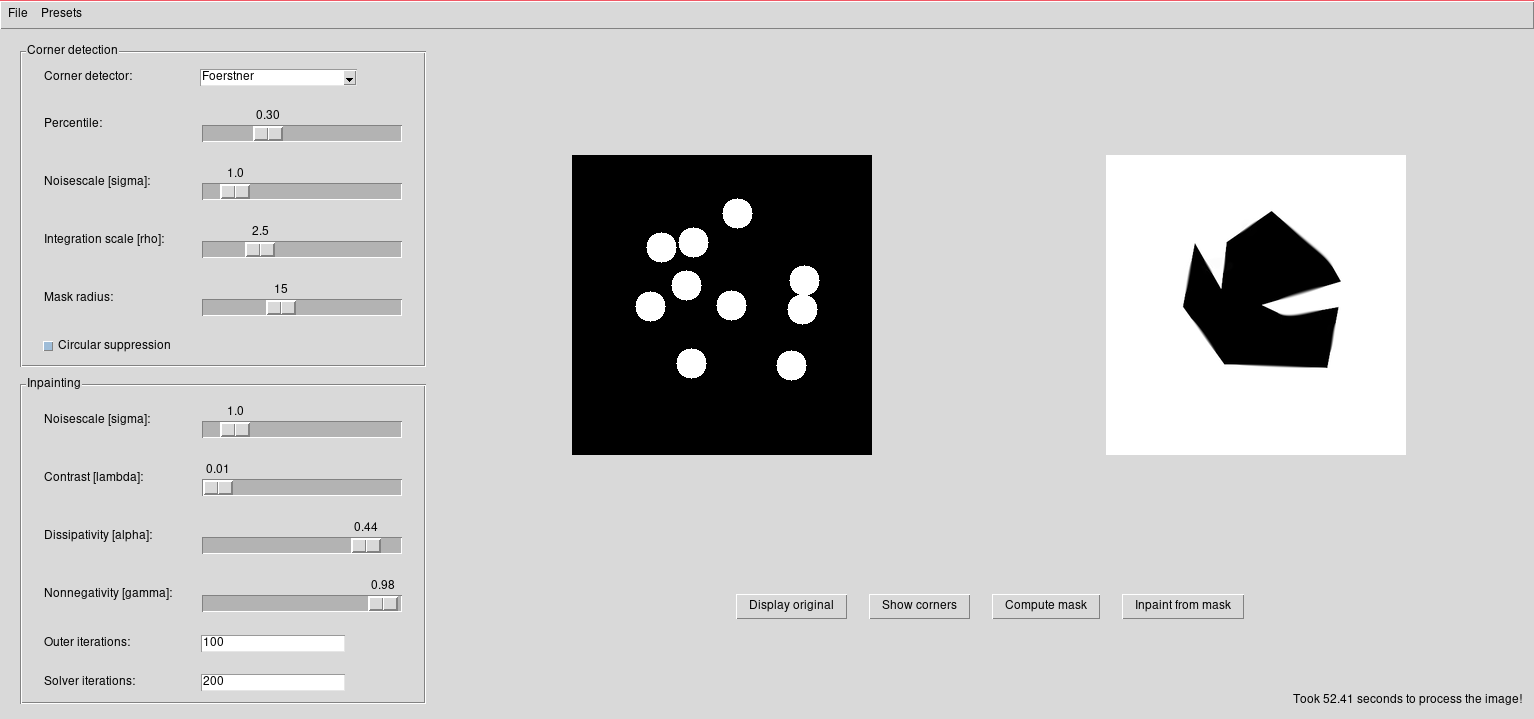
\includegraphics[width=\linewidth]{../Images/gui.png}
    \caption{GUI for easier testing}
\end{figure}
\begin{figure}
    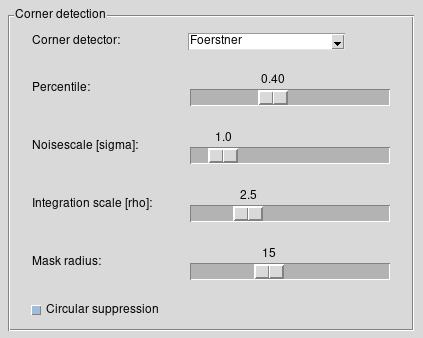
\includegraphics[width=0.5\linewidth]{../Images/parameters1.png}
    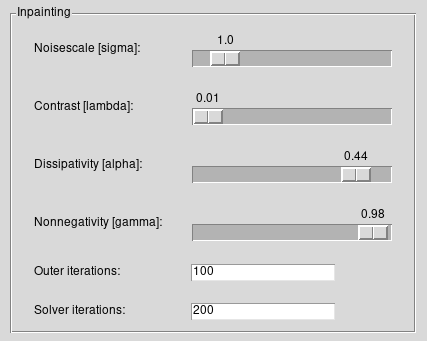
\includegraphics[width=0.5\linewidth]{../Images/parameters2.png}
    \caption{Panels to control parameters}
\end{figure}
